\section{Introduction}

Visual anomaly detection (VAD) is a prerequisite for safety in manufacturing, medical imaging, infrastructure inspection, and autonomous driving.
Recent work has explored using vision-language models (VLMs) for anomaly detection, leveraging their strong semantic reasoning capabilities~\citep{gu2024anomalygpt,jiang2024mmad,chen2026eagle}.
Yet three fundamental limitations prevent VLMs from serving as reliable cross-domain anomaly detectors.

\paragraph{Three VLM limitations in VAD.}
\emph{(1)~Lack of quantitative grounding.}
VLMs reason about visual content in natural language but cannot compute patch-level distance statistics that make expert detectors like PatchCore~\citep{roth2022patchcore} effective.
When a subtle surface scratch changes patch distances by 0.15 standard deviations, the VLM sees only pixels and may miss it entirely.
\emph{(2)~Hallucination and under-detection.}
Without quantitative anchoring, VLMs hallucinate defects on unfamiliar but normal images or fail to detect genuine anomalies when they lack domain-specific visual priors~\citep{jiang2024mmad}.
\emph{(3)~No self-verification.}
A single-pass VLM judgment has no mechanism to catch its own errors.
The model cannot revisit a claim when contradictory evidence emerges, nor can it request additional expert analysis when its initial assessment is uncertain.

Existing approaches address these limitations in isolation.
\emph{Vision-expert} methods~\citep{roth2022patchcore,oquab2024dinov2,jeong2023winclip} provide precise patch-level scores but cannot handle semantic or logical anomalies.
\emph{VLM-only} methods~\citep{gu2024anomalygpt,jiang2024mmad,cao2025anomalyonevision} reason fluently but lack quantitative grounding and self-correction.
Recent tool-augmented approaches~\citep{zhang2025agentiad,chen2026eagle,wei2025autoiad} combine VLMs with expert tools, but use fixed pipelines where the integration strategy is predetermined---the system cannot adapt its reasoning depth or expert selection based on the difficulty of each query.

\paragraph{Our approach: adversarial debate with expert grounding.}
AnomalyClaw addresses all three limitations through a principled framework built on three components (\Cref{fig:overview}).

First, an \textbf{extensible expert pool} provides quantitative grounding.
Rather than hardcoding a single expert (e.g., PatchCore), the framework supports a collection of lightweight analysis modules---patch-level nearest-neighbor scoring, visual retrieval, texture statistics, and others---each producing structured text evidence.
The expert pool is open: new experts can be added without modifying the debate engine.

Second, an \textbf{adversarial debate engine} enables self-verification.
An \emph{Anomaly Proposer} examines the query image alongside expert evidence and proposes specific anomaly claims---each with a spatial location, appearance description, and confidence level.
A \emph{Normality Advocate} then challenges each claim, arguing that the observation is a normal variation (lighting, texture, manufacturing tolerance) rather than a genuine anomaly.
Claims that survive refutation are accepted; those successfully challenged are rejected; ambiguous claims trigger additional debate rounds.
This adversarial structure forces the system to justify every detection against explicit counter-arguments, directly addressing the hallucination and self-verification problems.

Third, an \textbf{autonomous controller} orchestrates the process.
It determines which experts to invoke based on the initial assessment, controls debate depth (easy cases converge in one round; hard cases may require multiple), and manages the computational budget.
The controller replaces hand-crafted decision rules (e.g., family-specific fusion weights) with a self-regulating loop where the system dynamically allocates effort based on query difficulty.

\begin{figure}[t]
    \centering
    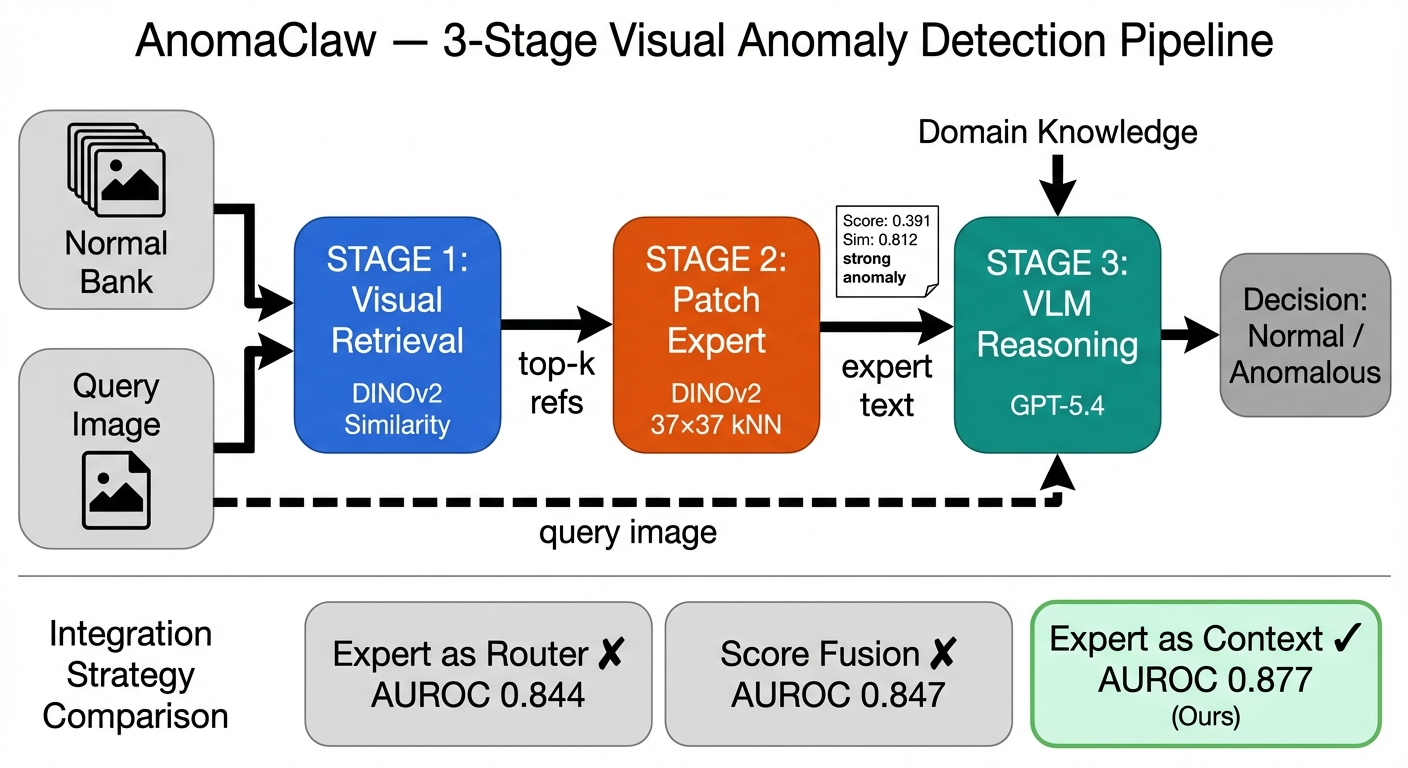
\includegraphics[width=0.95\linewidth]{figures/architecture.png}
    \caption{%
        \textbf{AnomalyClaw overview.}
        An extensible expert pool provides quantitative evidence (patch distances, retrieval similarity, texture statistics) as structured text.
        The Anomaly Proposer uses this evidence to identify potential defects with spatial locations and confidence scores.
        The Normality Advocate challenges each claim with counter-evidence (lighting variation, normal texture, manufacturing tolerance).
        An autonomous controller decides which experts to invoke, when to launch additional debate rounds, and when the system has converged.
    }
    \label{fig:overview}
\end{figure}

\paragraph{Contributions.}
\begin{enumerate}[leftmargin=*,itemsep=2pt,topsep=3pt]
    \item \textbf{Adversarial debate for anomaly detection.}
    We introduce an adversarial reasoning framework where an Anomaly Proposer and a Normality Advocate debate over each query image, grounded by expert evidence.
    This design provides built-in self-verification: every anomaly claim must survive explicit counter-arguments before being accepted.
    Ablations show that adversarial debate outperforms single-agent reasoning by \tbd{+X.X} AUROC points.

    \item \textbf{Extensible expert pool with autonomous invocation.}
    Expert evidence is provided through a modular pool of lightweight analysis modules (patch-level scoring, visual retrieval, texture analysis, etc.), selected and orchestrated by an autonomous controller that adapts to query difficulty.
    This replaces rigid pipeline designs with a self-regulating reasoning loop.

    \item \textbf{Cross-domain VAD benchmark.}
    We assemble a unified evaluation spanning 12 domains---industrial manufacturing (MVTec-AD), retail products (GoodsAD), complex and multi-object industrial inspection (VisA), infrastructure (SDNET2018), logical anomaly (MVTec-LOCO), 3D product inspection (Real3D-AD), satellite change detection (LEVIR-CD+), dermatology, brain MRI, liver CT, GI endoscopy, and road safety---comprising 1{,}440 test items with standardized metrics and protocols.

    \item \textbf{VLM-agnostic generalization.}
    We demonstrate that AnomalyClaw works across multiple VLM backends (\tbd{GPT-4o, GPT-5.4, open-source VLMs}) without modification, achieving consistent improvements over single-pass baselines regardless of the underlying model.
\end{enumerate}

The remainder of the paper is organized as follows.
\Cref{sec:related} reviews VLM-based and expert-based anomaly detection.
\Cref{sec:method} details the AnomalyClaw architecture.
\Cref{sec:experiments} presents experiments and ablations, and \Cref{sec:conclusion} concludes.
